\chapter[Análisis de Requisitos]{Análisis de Requisitos globales}

En este capítulos explicaremos el proceso de análisis de requisitos llevados a cabo para la elaboración de la aplicación y toda la información recibida por la comunidad así como las decisiones tomadas en base a otros proyectos similares al nuestro.

\section{Consultas con la comunidad}

A la hora de realizar las consultas con la comunidad hemos decidido ir a una charla de la ONCE para recabar información sobre las dificultades que los invidentes se encuentran a la hora de utilizar diferentes dispositivos y programas. 
También hemos preguntado a personas daltónicas para que nos guiaran sobre cómo se deberían de realizar juegos sin que ellos se vean afectados por su diseño.

Ambas consultas, así como el resultado obtenido de las mismas, se han especificado en la sección~\ref{sec:dificultadesfeedback} 

\subsection{Resumen de las peticiones recibidas}
	\paragraph{Fácil cambio de color de la interfaz} La interfaz gráfica tendrá diferentes colores que diferencien los distintos tipos de enemigos y elementos del juego. Tal y como hemos mencionado en la sección~\ref{sec:solventadodaltonicos}, deberíamos de tener esto en cuenta a pesar de que dichos elementos son fácilmente diferenciables.
	\paragraph{Descripciones automáticas de todos los elementos posibles} Las personas invidentes necesitan tener un feedback auditivo para saber qué es lo que está sucediendo y así poder tomar una decisión razonada en base a la situación en la que se encuentran. Debemos de generar estas descripciones de mejor manera posible para que no sean repetitivas. 
	\paragraph{Diferentes idiomas} Al ser un videojuego en el cual el idioma es esencial, debemos de tener en cuenta la inclusión de otras lenguas.
  \paragraph{Utilizar el idioma en nuestro favor} Usar elementos de temporalidad o diferentes adjetivos para definir ciertos elementos para que el lenguaje sea parte de la experiencia.
	\paragraph{Multiplataforma} Tal y como mencionamos en la introducción, nuestro software debe de poder ser ejecutado en varios sistemas operativos (Linux, Mac OS, Windows...).
	
\subsection{Cómo hemos abordado el problema de accesibilidad para invidentes en nuestro proyecto}

En el proyecto hemos creado descripciones para todos los elementos de la pantalla, por lo que el jugador siempre puede saber dónde se encuentra, qué hay a su alrededor, cuáles son sus características, las del enemigo y las de los elementos equipables, etc. También hemos creado una ventana que se encuentra al lado del juego y donde se van guardando todas las frases generadas, siendo la primera frase la última generada y leyéndose automáticamente por el reproductor de pantalla que esté siendo usado en ese momento (en nuestro caso se trata de \textit{NVDA}). De esta forma, una persona con visión siempre puede leer dicha frase mientras que el jugador invidente puede volver a escucharla las veces que quiera. Además de que el jugador también puede recordar lo sucedido anteriormente gracias a que los mensajes permanecen en la pantalla y pueden ser leidos por el lector de pantalla a usar.

\begin{figure}[H]
		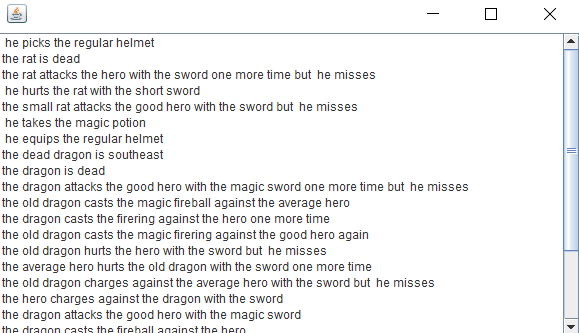
\includegraphics[width=\textwidth,height=\textheight,keepaspectratio]{./img/roomsGameTextArea.png}
	\caption{Captura de pantalla del area donde mostramos las frases generadas de nuestro juego para los invidentes}
	\label{fig:roomsgametextarea}
\end{figure}

\subsection{Cómo hemos solventado el problema en nuestro proyecto}
\label{sec:solventadodaltonicos}

En nuestro caso, al haber preguntado de antemano a los usuarios, siempre tuvimos desde el primer momento la idea de crear la interfaz gráfica con soporte para daltónicos en mente, a pesar de que, al haber tenido en cuenta a las personas invidentes, cualquier usuario podría jugarlo sin ninguna dificultad usando un lector de pantalla, de la misma forma que lo haría un jugador invidente.

Todos los elementos que se encuentran en la interfaz gráfica están diferenciados con caracteres completamente diferentes por lo que, incluso aunque todos los colores fueran iguales, sería sencillo identificar cada elemento por su forma en vez de por su color. 

De todas maneras, hemos creado una opción que cambia la paleta de colores a utilizar y facilita su visualización para aquellos usuarios que sufren de daltonismo.

\section{Análisis de los elementos del juego}
Al ser un \textit{roguelike}, debemos de incluir lo básico del género (aleatoriedad, dificultad, progreso, etc.). Los detalles de los mismos, así como lo que hemos introducido en el proyecto sobre ellos, se encuentran en la sección~\ref{sec:roguelikeinformacion}.

\section{Requisitos del aplicativo}
Con toda la información obtenida y analizada, creamos una lista con los casos de uso que nuestro proyecto debe de cumplir.

\begin{itemize}
  \item \textbf{Movimiento} Un usuario siempre será capaz de moverse con su personaje a una posición válida dentro de la habitación donde se encuentra. 
  \item \textbf{Ataque normal} Cuando el personaje está en la misma posición que un enemigo, éste será capaz de atacar cuerpo a cuerpo.
  \item \textbf{Ataque mágico} Cuando el personaje está a una distancia determinada del enemigo, éste será capaz de realizar un ataque mágico, siempre y cuando tenga sufiencience maná para el mismo. Si no, el ataque mágico se realizará, pero sin afectar a ningún enemigo (por lo que el usuario perderá maná).
  \item \textbf{Coger elemento} En las habitaciones del mapa habrá varios objetos que se pueden recolectar, así como enemigos que soltarán diferentes objetos.
  \item \textbf{Equipar elemento} Poder equipar un objeto que está en el inventario a nuestro personaje, siempre y cuando no tengamos un mismo objeto ya equipado.
  \item \textbf{Desequipar elemento} De la misma manera, podremos desequipar un objeto que tenemos equipado mientras tengamos espacio en el inventario.
  \item \textbf{Tirar elemento} En algunas ocasiones el jugador no tendrá suficiente espacio para almacenar nuevos elementos, por lo que se podrá tirar objetos del inventario para hacer hueco a aquellos nuevos que queramos recoger.
  \item \textbf{Descripciones} Durante el transcurso del juego podremos generar diferentes descripciones dependiendo de lo que queramos saber. Por ejemplo, lo que el usuario tiene en el inventario, las posiciones a las que nos podemos mover, la descripciones de los enemigos a los que nos enfrentamos, las propias estadísticas de él y de los enemigos, etc.
  \item \textbf{Activación de descripciones numéricas} Algunas de las descripciones nos comentarán posiciones o características de los enemigos que podremos querer escuchar numéricamente (por ejemplo la cantidad de vida de un cierto monstruo) o con palabras (mucha, poca, bastante...), dependiendo de lo que prefiramos.
  \item \textbf{Cambio de colores} Para gente que es daltónica hemos incluido una opción para cambiar el color de la interfaz gráfica.
\end{itemize}

Al realizar algunas de estas acciones (coger, equipar, desequipar y tirar un objeto, moverse y atacar), un turno será consumido. Al consumir un turno los enemigos realizarán el suyo, por lo que el jugador puede ser atacado o enemigos pueden acercarse a él.

\begin{figure}[h!]
    \centering
    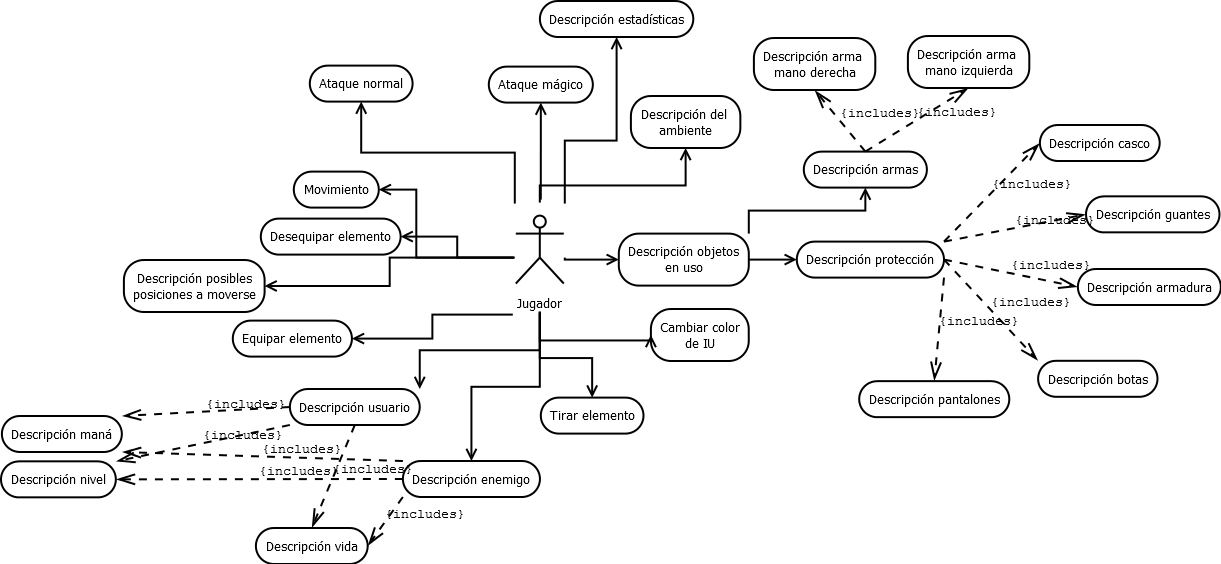
\includegraphics[width=0.9\textheight,angle=90]{img/casosdeuso.png}
    \caption{Diagrama UML de casos de uso del proyecto}
    \label{fig:casosdeuso}
\end{figure}